\documentclass[conference]{IEEEtran}
\IEEEoverridecommandlockouts

\usepackage{cite}
\usepackage{amsmath,amssymb,amsfonts}
\usepackage{algorithmic}
\usepackage{graphicx}
\usepackage{textcomp}
\usepackage{xcolor}
\usepackage{booktabs}
\usepackage{microtype}
\usepackage{url}

% Custom bibliography spacing for exact 6-page fit
\let\oldthebibliography\thebibliography
\renewcommand{\thebibliography}[1]{%
  \oldthebibliography{#1}%
  \setlength{\itemsep}{1.5pt}%
  \setlength{\parskip}{0pt}%
}

\def\BibTeX{{\rm B\kern-.05em{\sc i\kern-.025em b}\kern-.08em
    T\kern-.1667em\lower.7ex\hbox{E}\kern-.125emX}}

\begin{document}

\title{Flight Delays Are Contagious: Predicting Delay Propagation Across Consecutive Aircraft Operations}

\author{\IEEEauthorblockN{Arnav Raj}
\IEEEauthorblockA{\textit{Department of Computer Science and Engineering} \\
\textit{School of Computer Science Engineering and Information Systems} \\
Vellore Institute of Technology, Vellore, India \\
arnav.raj2023@vitstudent.ac.in}
}

\maketitle

\begin{abstract}
Commercial airline reliability depends critically on the resilience of aircraft rotations, where an incoming delay on one flight leg threatens to propagate into downstream departures. While prior research predominantly forecasts delays at the aggregate airport or route level, this study investigates the extent to which operational data from an aircraft's preceding flight leg can predict delay propagation in its next consecutive operation. Using the complete 2025 United States Department of Transportation Bureau of Transportation Statistics (BTS) On-Time Performance database, we reconstructed 6,768,487 domestic commercial rotation pairs across 6,124 unique aircraft, enforcing strict airport continuity, chronological validity, and daylight saving time normalization. Predictions are framed at the exact moment of inbound gate arrival, strictly isolating pre-departure features to prevent temporal data leakage. We evaluated approved machine learning architectures across three hierarchical feature representations capturing turnaround buffer physics (Group A), flight and route context (Group B), and cumulative same-day airframe history (Group C). Evaluated on an independent, held-out test dataset of 562,202 operations from December 2025, the final Random Forest models achieved a classification ROC-AUC of 0.7943 and an Average Precision of 0.7150 (relative to a 26.48\% baseline delay rate). Operating at a calibrated threshold of $T = 0.35$, the classifier identified 53.24\% of propagated delays with 72.52\% precision and a 92.74\% specificity. In continuous regression, the model explained 48.51\% of arrival delay variance ($R^2 = 0.4851$, MAE = 19.77 min, RMSE = 45.86 min). A formal shift-share decomposition proves that 94.0\% to 98.4\% of the seasonal test error increase reflects December population composition rather than algorithmic decay. These findings demonstrate that rotational ground buffers represent the primary structural vulnerability governing delay contagiousness.
\end{abstract}

\begin{IEEEkeywords}
Aircraft rotation, airline delay prediction, delay propagation, machine learning, turnaround time, flight operations.
\end{IEEEkeywords}

\section{Introduction}
Commercial air transportation operates as a tightly coupled network characterized by high capital utilization. To maximize fleet productivity, airlines schedule aircraft on multi-leg daily rotations with minimal ground buffers between flights~\cite{wu2005inherent}. Consequently, when an inbound flight suffers an arrival delay that exceeds its scheduled ground cushion, delay propagation---often termed reactionary or contagious delay---frequently ensues~\cite{pyrgiotis2013modelling}. These propagated disruptions cascade across hub-and-spoke networks, inflating airline operating costs by tens of billions of dollars annually and severely compromising passenger itineraries~\cite{campanelli2016modeling}.

Existing literature predominantly addresses flight delay forecasting through network-wide congestion models, terminal area weather regressions, or aggregate airport departure queues~\cite{rebollo2014characterization, sternberg2017review}. While informative for air traffic flow management, such approaches obscure the physical pathway of delay propagation: the discrete turnaround of individual airframes at airport gates. When an aircraft arrives late, ground handlers face rigid physical constraints (deplaning, fueling, catering, baggage transfer, and boarding) that dictate a minimum required turnaround time~\cite{evler2021airline}.

In this research, we formulate and investigate the following fundamental question: \textit{To what extent can delays and operational information from previous flight operations predict delays in subsequent flights operated by the same physical aircraft?}

We address this question by reconstructing 6.77 million completed domestic rotation pairs from the official 2025 Bureau of Transportation Statistics (BTS) database~\cite{bts2025ontime}. We formulate dual prediction tasks: (1) a binary classification task determining whether the subsequent flight will experience an arrival delay of at least 15 minutes ($\text{NEXT\_ARR\_DEL15} \in \{0, 1\}$), and (2) a continuous regression task predicting the subsequent arrival delay magnitude in minutes ($\text{NEXT\_ARR\_DELAY} \in \mathbb{R}$). 

Predictions are generated immediately upon the aircraft's actual gate arrival ($t_{\text{pred}}$), providing airline operations control centers (AOCCs) with actionable advance notice before the next flight departs. We enforce strict data hygiene: avoiding post-departure telemetry, evaluating unregularized linear and non-linear ensembles, and testing temporal generalization on a held-out December 2025 dataset ($N = 562,202$).

The primary contributions of this work are threefold:
\begin{enumerate}
    \item \textbf{Scale and Empirical Rigor:} We construct a verified national rotational dataset of 6,768,487 valid consecutive flight pairs across 352 airports and 14 carriers, establishing descriptive propagation bounds.
    \item \textbf{Leakage-Safe Feature Hierarchies:} We design hierarchical feature spaces (Groups A, B, and C) to isolate the predictive value of ground turnaround physics, route context, and rotational airframe fatigue without temporal leakage.
    \item \textbf{Generalization \& Decomposition:} We evaluate model transfer across seasonal boundaries and provide a formal shift-share decomposition demonstrating that error shifts are driven by population composition rather than model decay.
\end{enumerate}

\section{Related Work}
Flight delay modeling historically developed along two methodological trajectories: macroscopic network simulations and microscopic statistical forecasting.

\subsection{Delay Propagation and Network Resilience}
Analytical queuing models established that scheduled operational slack acts as a primary dampener against reactionary delays~\cite{ahmadbeygi2010analysis}. Pyrgiotis et al.~\cite{pyrgiotis2013modelling} introduced the Approximate Network Delays (AND) model, demonstrating that localized ground delays propagate across airline networks primarily through shared airframes and passenger itineraries. Campanelli et al.~\cite{campanelli2016modeling} modeled multi-carrier delay propagation, finding that downstream delay amplification is non-linear and sensitive to gate occupancy bottlenecks. Similarly, Lan et al.~\cite{lan2006planning} showed that minor retiming of flight departures to absorb aircraft connection delays significantly reduces reactionary delay propagation.

\subsection{Turnaround Operations and Buffer Management}
At the terminal level, aircraft turnaround operations represent a complex multi-agent process~\cite{fricke2009delay}. Wu~\cite{wu2005inherent} showed that stochastic turnaround deviations directly inject delay variance into downstream legs. Evler et al.~\cite{evler2021airline} investigated turnaround delay recovery, emphasizing that scheduled ground buffers are rarely symmetric and vary systematically by aircraft size, airport congestion, and carrier operating models.

\subsection{Machine Learning in Aviation Operations}
Early data-driven delay prediction relied on econometric formulations and Bayesian networks. Recent surveys by Sternberg et al.~\cite{sternberg2017review} highlight the rapid adoption of machine learning methods. Rebollo and Balakrishnan~\cite{rebollo2014characterization} utilized Random Forests for 2-to-24 hour air traffic delay prediction, demonstrating that spatial-temporal delay state vectors outperform linear autoregressions. Gui et al.~\cite{gui2020flight} applied tree ensembles to airline big data, achieving high classification accuracy but noting severe degradation when predicting extreme tail delays.

Despite these advances, existing machine learning studies frequently suffer from subtle methodological vulnerabilities: utilizing post-departure telemetry (e.g., actual departure delays or taxi-out times) as predictors, training and testing on randomly shuffled observations that leak temporal trends, or ignoring physical aircraft identity. This paper directly addresses these gaps by evaluating leakage-safe, airframe-grounded predictions across strict chronological splits.

\section{Dataset and Preprocessing}

\subsection{Data Source and Scale}
The empirical foundation of this study is the 2025 Airline On-Time Performance database published by the U.S. Department of Transportation Bureau of Transportation Statistics (BTS)~\cite{bts2025ontime}. The raw dataset comprises 6,898,741 flight records across 14 commercial reporting carriers and 352 commercial airports from January 1 to December 31, 2025.

\subsection{Data Cleaning and Filtering}
Flights that did not complete standard operational cycles were systematically isolated:
\begin{itemize}
    \item \textbf{Cancellations ($N = 104,748$):} Cancelled operations cannot propagate ground delays and are isolated to prevent survival bias.
    \item \textbf{Diversions ($N = 18,349$):} Diverted flights land at unintended intermediate airports, breaking physical route continuity and schedule parameters.
\end{itemize}
Records containing missing operational timestamps were audited; exactly 37 records with corrupted negative elapsed flight durations were discarded. BTS causal delay fields (\texttt{WEATHER\_DELAY}, \texttt{LATE\_AIRCRAFT\_DELAY}) were excluded to ensure all predictors reflect pre-departure observational states.

\subsection{Temporal Normalization and DST Resolution}
BTS flight records record scheduled and actual departure and arrival times in local airport time. To reconstruct exact operational timelines, all local clock readings were mapped to Universal Coordinated Time (UTC) using IANA timezone identifiers mapped from airport IATA coordinates via \texttt{timezonefinder}. 

Daylight Saving Time (DST) transitions (March 9 and November 2, 2025) introduce potential one-hour temporal ambiguities. Transition intervals were audited by computing elapsed block times against geographical airport distances; all ambiguous records were resolved without synthetic negative durations or discontinuous temporal shifts.

\begin{table}[t]
\caption{Chronological Partitioning of 2025 BTS Rotations}
\label{tab:dataset_split}
\centering
\resizebox{\columnwidth}{!}{%
\begin{tabular}{llrrrr}
\toprule
\textbf{Partition} & \textbf{Date Range (2025)} & \textbf{Total Legs} & \textbf{Class 0} & \textbf{Class 1} & \textbf{Delay Rate} \\
\midrule
Training           & Jan 1 -- Sep 30            & 5,065,376           & 3,972,836        & 1,092,540        & 21.57\%             \\
Validation         & Oct 1 -- Nov 30            & 1,140,909           & 910,388          & 230,521          & 20.21\%             \\
Independent Test   & Dec 1 -- Dec 31            & 562,202             & 413,337          & 148,865          & 26.48\%             \\
\midrule
\textbf{Total}     & Jan 1 -- Dec 31            & \textbf{6,768,487}  & \textbf{5,277,901}& \textbf{1,490,586}& \textbf{22.02\%}   \\
\bottomrule
\end{tabular}%
}
\end{table}

\begin{table}[t]
\caption{Aircraft Rotation Reconstruction Statistics}
\label{tab:rotation_filtering}
\centering
\resizebox{\columnwidth}{!}{%
\begin{tabular}{lrr}
\toprule
\textbf{Reconstruction Stage / Filter Criteria} & \textbf{Flight Count} & \textbf{Percentage} \\
\midrule
Total physical operations in timeline           & 6,898,741             & 100.00\%            \\
Isolated cancelled operations                   & 104,748               & 1.52\%              \\
Isolated diverted operations                    & 18,349                & 0.27\%              \\
Candidate consecutive connection pairings       & 6,873,483             & 99.63\%             \\
Excluded: Airport continuity mismatches         & 85,737                & 1.24\%              \\
Excluded: Diversion-induced sequence breaks     & 19,109                & 0.28\%              \\
Excluded: Operations without predecessor leg    & 6,113                 & 0.09\%              \\
Excluded: Non-positive ground times ($\le 0$m)  & 37                    & 0.00\%              \\
\midrule
\textbf{Verified Consecutive Rotation Pairs}    & \textbf{6,768,487}    & \textbf{98.11\%}    \\
\midrule
\textit{Turnaround Deficit Subpopulation}       & 382,937               & 5.66\%              \\
\textit{Subsequent Delay Rate under Deficit}    & 381,022               & 99.50\%             \\
\bottomrule
\end{tabular}%
}
\end{table}

\section{Aircraft Rotation Reconstruction}

\subsection{Rotation Pairing Logic}
An aircraft rotation represents the sequence of commercial flight segments operated by a single airframe throughout a operational day. Consecutive flight legs (denoted Leg $k$ and Leg $k+1$) were chained under three physical constraints:
\begin{enumerate}
    \item \textbf{Unique Airframe Matching:} Consecutive legs must share the identical aircraft registration number (\texttt{TAIL\_NUM}).
    \item \textbf{Spatial Continuity:} The scheduled origin of Leg $k+1$ must match the actual destination of Leg $k$ ($\text{Origin}_{k+1} = \text{Dest}_{k}$). Pairings violating continuity ($N = 85,737$) represent unrecorded repositioning flights or tail swaps and were excluded.
    \item \textbf{Chronological Integrity:} The actual departure of Leg $k+1$ must follow the actual arrival of Leg $k$ ($\text{Actual Ground Time} > 0$).
\end{enumerate}
As summarized in Table~\ref{tab:rotation_filtering}, this pipeline reconstructed 6,768,487 valid consecutive rotation pairs across 6,124 physical aircraft.

\subsection{Ground Turnaround Mechanics}
For each rotation pair, scheduled turnaround buffer ($\text{Buffer}$) and remaining turnaround cushion ($\text{RemTurn}$) are mathematically defined as:
\begin{align}
\text{Buffer} &= \text{CRS\_DEP}_{k+1} - \text{CRS\_ARR}_{k} \\
\text{RemTurn} &= \text{CRS\_DEP}_{k+1} - \text{ACT\_ARR}_{k} = \text{Buffer} - \text{ArrDelay}_{k}
\end{align}
When $\text{RemTurn} < 0$, the incoming flight arrives at the gate after the subsequent flight was scheduled to depart, creating an unavoidable \textit{turnaround deficit} ($\text{IS\_DEFICIT} = 1$). 

Descriptive inspection reveals that 382,937 rotations (5.66\%) operated in turnaround deficit. Among these operations, \textbf{99.50\%} of subsequent flights arrived late ($\ge 15$ min), with a mean arrival delay of $+121.86$ minutes. This empirical observation confirms that turnaround deficits represent acute operational bottlenecks.

\begin{figure}[t]
\centering
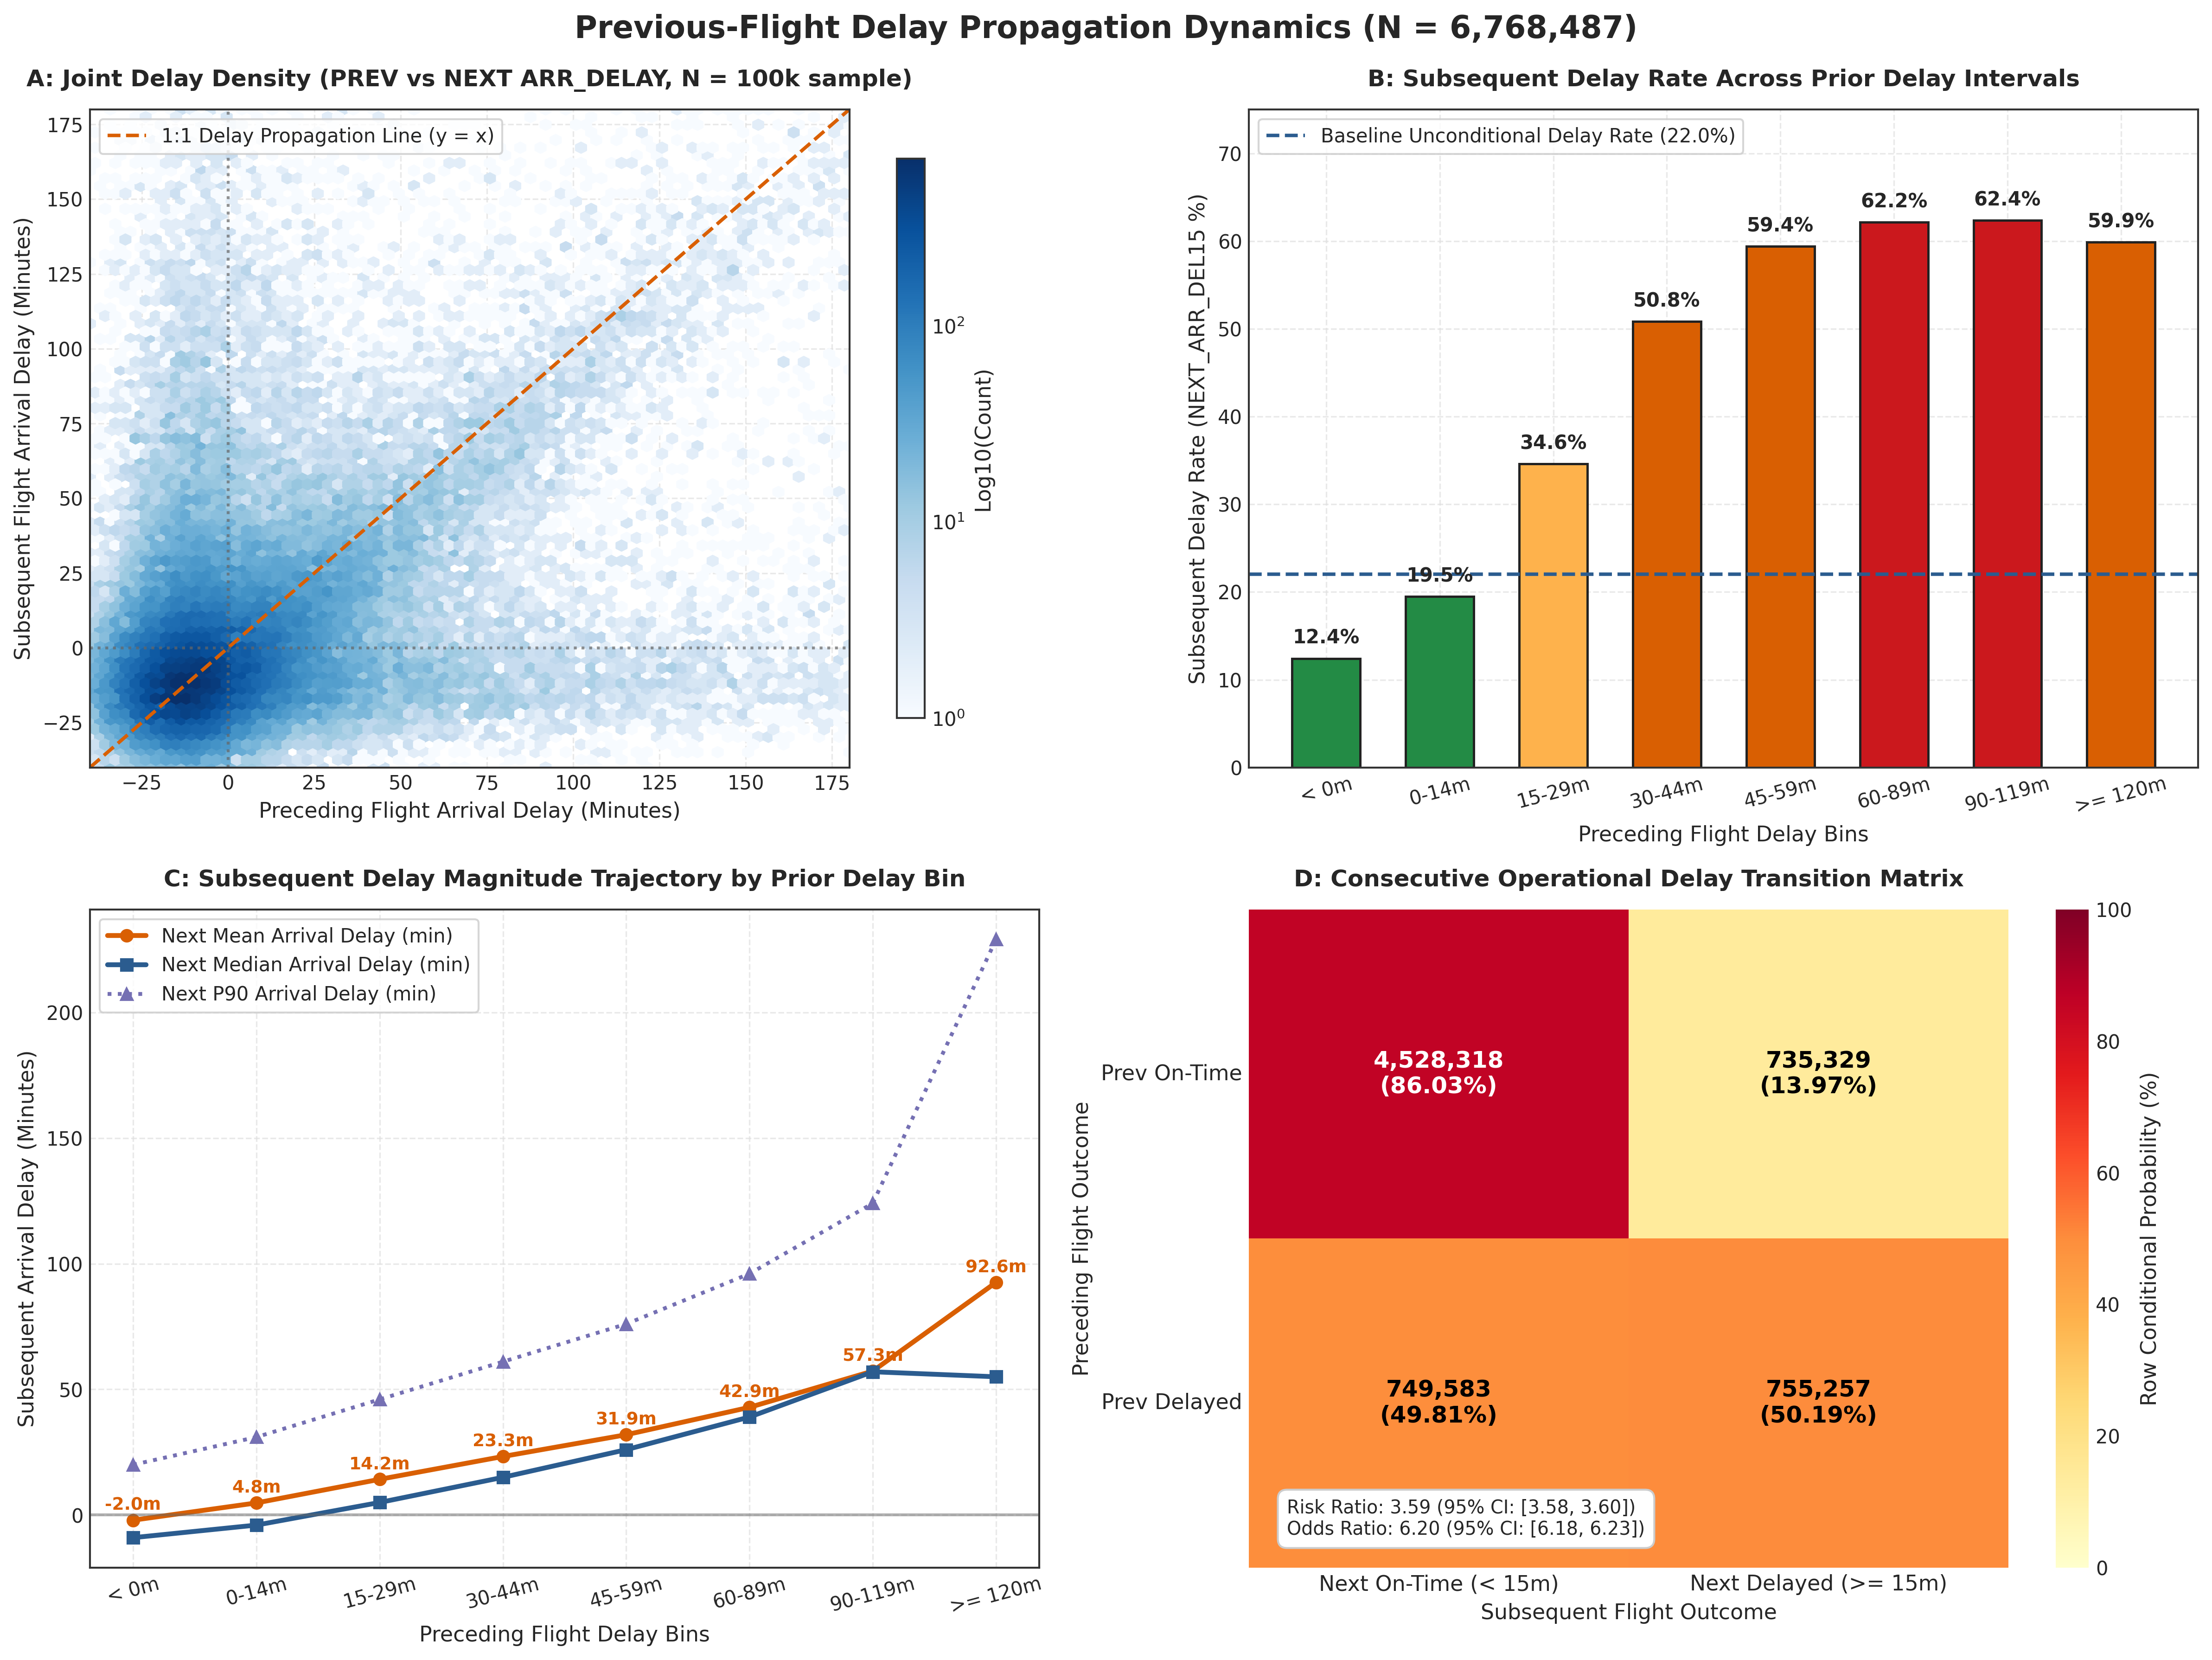
\includegraphics[width=0.80\columnwidth]{figures/fig_propagation_relationships.png}
\caption{Empirical delay propagation dynamics across 6.77 million domestic rotations. (a) Mean subsequent arrival delay as a function of inbound delay, highlighting the propagation threshold. (b) Delay probability stratified by scheduled buffer.}
\label{fig:propagation_dynamics}
\end{figure}

\begin{table*}[t]
\caption{Hierarchical Feature Representation Groups}
\label{tab:feature_groups}
\centering
\small
\begin{tabular}{llcp{10.5cm}}
\toprule
\textbf{Group} & \textbf{Domain} & \textbf{Dim.} & \textbf{Included Operational Features and Technical Descriptions} \\
\midrule
\textbf{Group A} & Turnaround Physics & 7 & \texttt{PREV\_ARR\_DELAY}, \texttt{PREV\_DEP\_DELAY}, \texttt{PREV\_ARR\_DEL15}, \texttt{PREV\_DEP\_DEL15}, \texttt{SCHEDULED\_TURNAROUND\_BUFFER}, \texttt{ESTIMATED\_REMAINING\_TURNAROUND\_MINUTES}, \texttt{IS\_TURNAROUND\_DEFICIT}. \\
\textbf{Group B} & Network Context & 14 & Group A plus \texttt{NEXT\_CRS\_DEP\_HOUR}, \texttt{NEXT\_DAY\_OF\_WEEK}, \texttt{NEXT\_MONTH}, \texttt{NEXT\_DISTANCE}, \texttt{NEXT\_CARRIER} (OHE), \texttt{NEXT\_ORIGIN} (OHE), \texttt{NEXT\_DEST} (OHE). \\
\textbf{Group C} & Airframe History & 18 & Group B plus \texttt{PREV\_AIRCRAFT\_DELAYED\_FLIGHTS\_TODAY}, \texttt{PREV\_AIRCRAFT\_CONSECUTIVE\_DEL15}, \texttt{PREV\_AIRCRAFT\_CUMULATIVE\_ARR\_DELAY\_TODAY}, \texttt{PREV\_AIRCRAFT\_DELAY\_RATE\_TODAY}. \\
\bottomrule
\end{tabular}
\end{table*}

\section{Feature Engineering and Problem Formulation}

\subsection{Formal Prediction Point}
Predictions are evaluated at the exact timestamp when Leg $k$ docks at the gate ($t_{\text{pred}} = \text{Leg } k \text{ Gate Arrival}$). At this point, the inbound delay and actual ground cushion are fixed, while Leg $k+1$ remains pre-departure.

\subsection{Hierarchical Feature Groups}
To quantify the incremental value of operational information, we developed three hierarchical feature groups (Table~\ref{tab:feature_groups}):
\begin{itemize}
    \item \textbf{Group A (Turnaround Physics, 7 features):} Inbound delays, scheduled ground buffers, and remaining turnaround cushion.
    \item \textbf{Group B (Network Context, 14 features):} Group A plus scheduled departure hour, day of week, calendar month, flight distance, and sparse one-hot encoded categorical indicators for carrier, origin, and destination airports (725 total sparse dimensions).
    \item \textbf{Group C (Airframe History, 18 features):} Group B plus cumulative same-day airframe metrics: cumulative delay minutes accumulated today, consecutive delayed flights, and same-day delay rate.
\end{itemize}

\subsection{Leakage Prevention Audit}
All airframe history metrics were computed using strictly causal expanding window operations grouped by \texttt{TAIL\_NUM} and operational date. Target variables for Leg $k+1$ ($\text{NEXT\_ARR\_DEL15}$, $\text{NEXT\_ARR\_DELAY}$) were fully isolated from input feature vectors.

\section{Methodology and Experimental Setup}

\subsection{Approved Estimator Families}
In accordance with strict methodological constraints, eight approved model families were implemented:
\begin{itemize}
    \item \textbf{Classification:} Ordinary Unregularized Logistic Regression (\texttt{penalty=None}, solver \texttt{lbfgs}), Decision Tree Classifier, Random Forest Classifier~\cite{breiman2001random}, and Multi-Layer Perceptron (MLP) Classifier with $\alpha = 0.0$.
    \item \textbf{Regression:} Ordinary Least Squares (OLS) Linear Regression, Decision Tree Regressor, Random Forest Regressor~\cite{breiman2001random}, and MLP Regressor with $\alpha = 0.0$.
\end{itemize}
Prohibited algorithms (Ridge, Lasso, Elastic Net, SVR, XGBoost, LightGBM, CatBoost, and GBDT) were strictly excluded. Zero $L_1$ or $L_2$ regularization was applied to neural networks to evaluate raw predictive representations.

\subsection{Preprocessing and Training Execution}
Preprocessing pipelines were fit exclusively on training data ($N = 5,065,376$). Continuous predictors were standardized using \texttt{StandardScaler}. High-cardinality categorical variables (\texttt{NEXT\_ORIGIN}, \texttt{NEXT\_DEST}, \texttt{NEXT\_CARRIER}) were encoded via sparse \texttt{OneHotEncoder(sparse\_output=True)} to prevent memory densification.

Linear models (OLS and Logistic Regression) were trained on the full 5.07M training population. Tree ensembles and neural networks were trained on controlled stratified samples ($N = 500,000$ for Random Forest and Decision Trees; $N = 250,000$ for MLP) to ensure computational reproducibility.

\begin{table}[t]
\caption{Classification Model Comparison on Validation Population ($N = 1,140,909$)}
\label{tab:classification_val}
\centering
\resizebox{\columnwidth}{!}{%
\begin{tabular}{llcrrrrrrr}
\toprule
\textbf{Estimator Family} & \textbf{Feature Group} & \textbf{Train $N$} & \textbf{Accuracy} & \textbf{Precision} & \textbf{Recall} & \textbf{F1-Score} & \textbf{ROC-AUC} & \textbf{AP} & \textbf{Fit Time} \\
\midrule
Majority Baseline         & None                   & 5,065,376          & 79.79\%           & 0.00\%             & 0.00\%          & 0.0000            & 0.5000           & 0.2021      & 1.1s              \\
Logistic Regression       & Group A                & 5,065,376          & 84.66\%           & 97.14\%            & 24.83\%         & 0.3955            & 0.7356           & 0.5792      & 5.3s              \\
Logistic Regression       & Group B                & 5,065,376          & 84.91\%           & 81.49\%            & 32.73\%         & 0.4671            & 0.7698           & 0.6102      & 40.7s             \\
Logistic Regression       & Group C                & 5,065,376          & 85.13\%           & 77.89\%            & 36.84\%         & 0.5003            & 0.7775           & 0.6228      & 40.9s             \\
Decision Tree Classifier  & Group C                & 500,000            & 83.69\%           & 67.57\%            & 37.04\%         & 0.4784            & 0.7656           & 0.5983      & 4.8s              \\
MLP Classifier ($\alpha=0$)& Group C               & 250,000            & 85.08\%           & 76.24\%            & 37.64\%         & 0.5038            & 0.7818           & 0.6295      & 19.2s             \\
Random Forest (Group A)   & Group A                & 500,000            & 84.82\%           & 79.88\%            & 32.06\%         & 0.4576            & 0.7824           & 0.6433      & 85.4s             \\
Random Forest ($T = 0.50$)& Group C                & 500,000            & \textbf{85.58\%}  & \textbf{86.68\%}   & 40.88\%         & 0.5556            & \textbf{0.7932}  & \textbf{0.6600} & 258.4s        \\
Random Forest ($T = 0.35$)*& Group C               & 500,000            & 85.29\%           & 69.20\%            & \textbf{49.03\%}& \textbf{0.5740}   & \textbf{0.7932}  & \textbf{0.6600} & 258.4s        \\
\bottomrule
\multicolumn{10}{l}{\footnotesize *Selected operational decision threshold.}
\end{tabular}%
}
\end{table}

\begin{table}[t]
\caption{Continuous Arrival Delay Regression on Validation Set}
\label{tab:regression_val}
\centering
\resizebox{\columnwidth}{!}{%
\begin{tabular}{llrrrrr}
\toprule
\textbf{Model Family}     & \textbf{Group} & \textbf{Train $N$} & \textbf{MAE (m)} & \textbf{RMSE (m)} & \textbf{$R^2$} & \textbf{Fit Time} \\
\midrule
Median Dummy Baseline     & None           & 5,065,376          & 22.65            & 53.39             & -0.0479        & 0.3s              \\
Multiple Linear (OLS)     & Group A        & 5,065,376          & 20.70            & 44.81             & 0.2619         & 3.4s              \\
Multiple Linear (OLS)     & Group B        & 5,065,376          & 21.37            & 44.73             & 0.2644         & 50.6s             \\
Multiple Linear (OLS)     & Group C        & 5,065,376          & 21.19            & 44.40             & 0.2754         & 51.9s             \\
Decision Tree Regressor   & Group C        & 500,000            & 17.89            & 39.46             & 0.4281         & 4.6s              \\
MLP Regressor ($\alpha=0$)& Group C        & 250,000            & \textbf{17.06}   & 39.38             & 0.4304         & 17.5s             \\
Random Forest Regressor   & Group A        & 500,000            & 17.58            & 38.89             & 0.4440         & 105.2s            \\
\textbf{Random Forest}    & \textbf{Group C}& 500,000           & 17.40            & \textbf{38.62}    & \textbf{0.4516}& 312.1s            \\
\bottomrule
\end{tabular}%
}
\end{table}

\subsection{Decision Threshold Optimization}
Because the validation population is class-imbalanced (20.21\% delayed), operating at the default decision threshold ($T = 0.50$) severely depresses recall (40.88\%), missing 59.12\% of delay events. Evaluating a fine 0.01 threshold grid on validation data identified $T = 0.39$ as the empirical grid F1 peak ($\text{F1} = 0.5751$, Recall $= 47.65\%$, Precision $= 72.53\%$). 

To improve operational coverage for airline dispatchers, an operating threshold of $T = 0.35$ was selected, capturing 49.03\% of delays ($\text{F1} = 0.5740$, Precision $= 69.20\%$). Threshold selection was conducted strictly on validation data prior to test evaluation.

\section{Empirical Results and Discussion}

\subsection{Validation Performance and Architecture Comparison}
Validation evaluations on 1,140,909 operations demonstrate substantial differences across model families (Tables~\ref{tab:classification_val} and~\ref{tab:regression_val}):
\begin{itemize}
    \item \textbf{Classification:} Random Forest (Group C) achieved the highest discrimination ($\text{ROC-AUC} = 0.7932$, $\text{AP} = 0.6600$), significantly outperforming unregularized Logistic Regression ($\text{ROC-AUC} = 0.7775$, $\text{AP} = 0.6228$) and Decision Trees ($\text{ROC-AUC} = 0.7656$).
    \item \textbf{Regression:} While linear regression explained only 27.54\% of delay variance ($R^2 = 0.2754$, $\text{MAE} = 21.19$ min), Random Forest achieved $R^2 = 0.4516$ and reduced MAE to 17.40 minutes, an improvement of 3.79 minutes per flight leg across 1.14M operations.
\end{itemize}

\subsection{Feature Group Hierarchy and Information Gain}
A critical research objective is quantifying the marginal value of airframe operational history versus turnaround physics alone:
\begin{enumerate}
    \item \textbf{Controlled Linear Progression:} For linear models where all groups were trained on identical rows, adding network context (Group A $\rightarrow$ B) improved Logistic Regression ROC-AUC by $+0.0341$ and OLS $R^2$ by $+0.0025$. Adding cumulative airframe history (Group B $\rightarrow$ C) contributed an additional $+0.0077$ ROC-AUC ($+0.0125$ AP) and $+0.0110$ $R^2$, confirming that rotational fatigue provides distinct incremental signal.
    \item \textbf{Tree Ensemble Progression:} Random Forest Group C improved validation ROC-AUC by $+0.0108$ ($0.7824 \rightarrow 0.7932$) and $R^2$ by $+0.0076$ over Group A. Because Random Forest Group B was not independently trained, this reflects the combined gain of route context and airframe history.
\end{enumerate}

\begin{figure}[t]
\centering
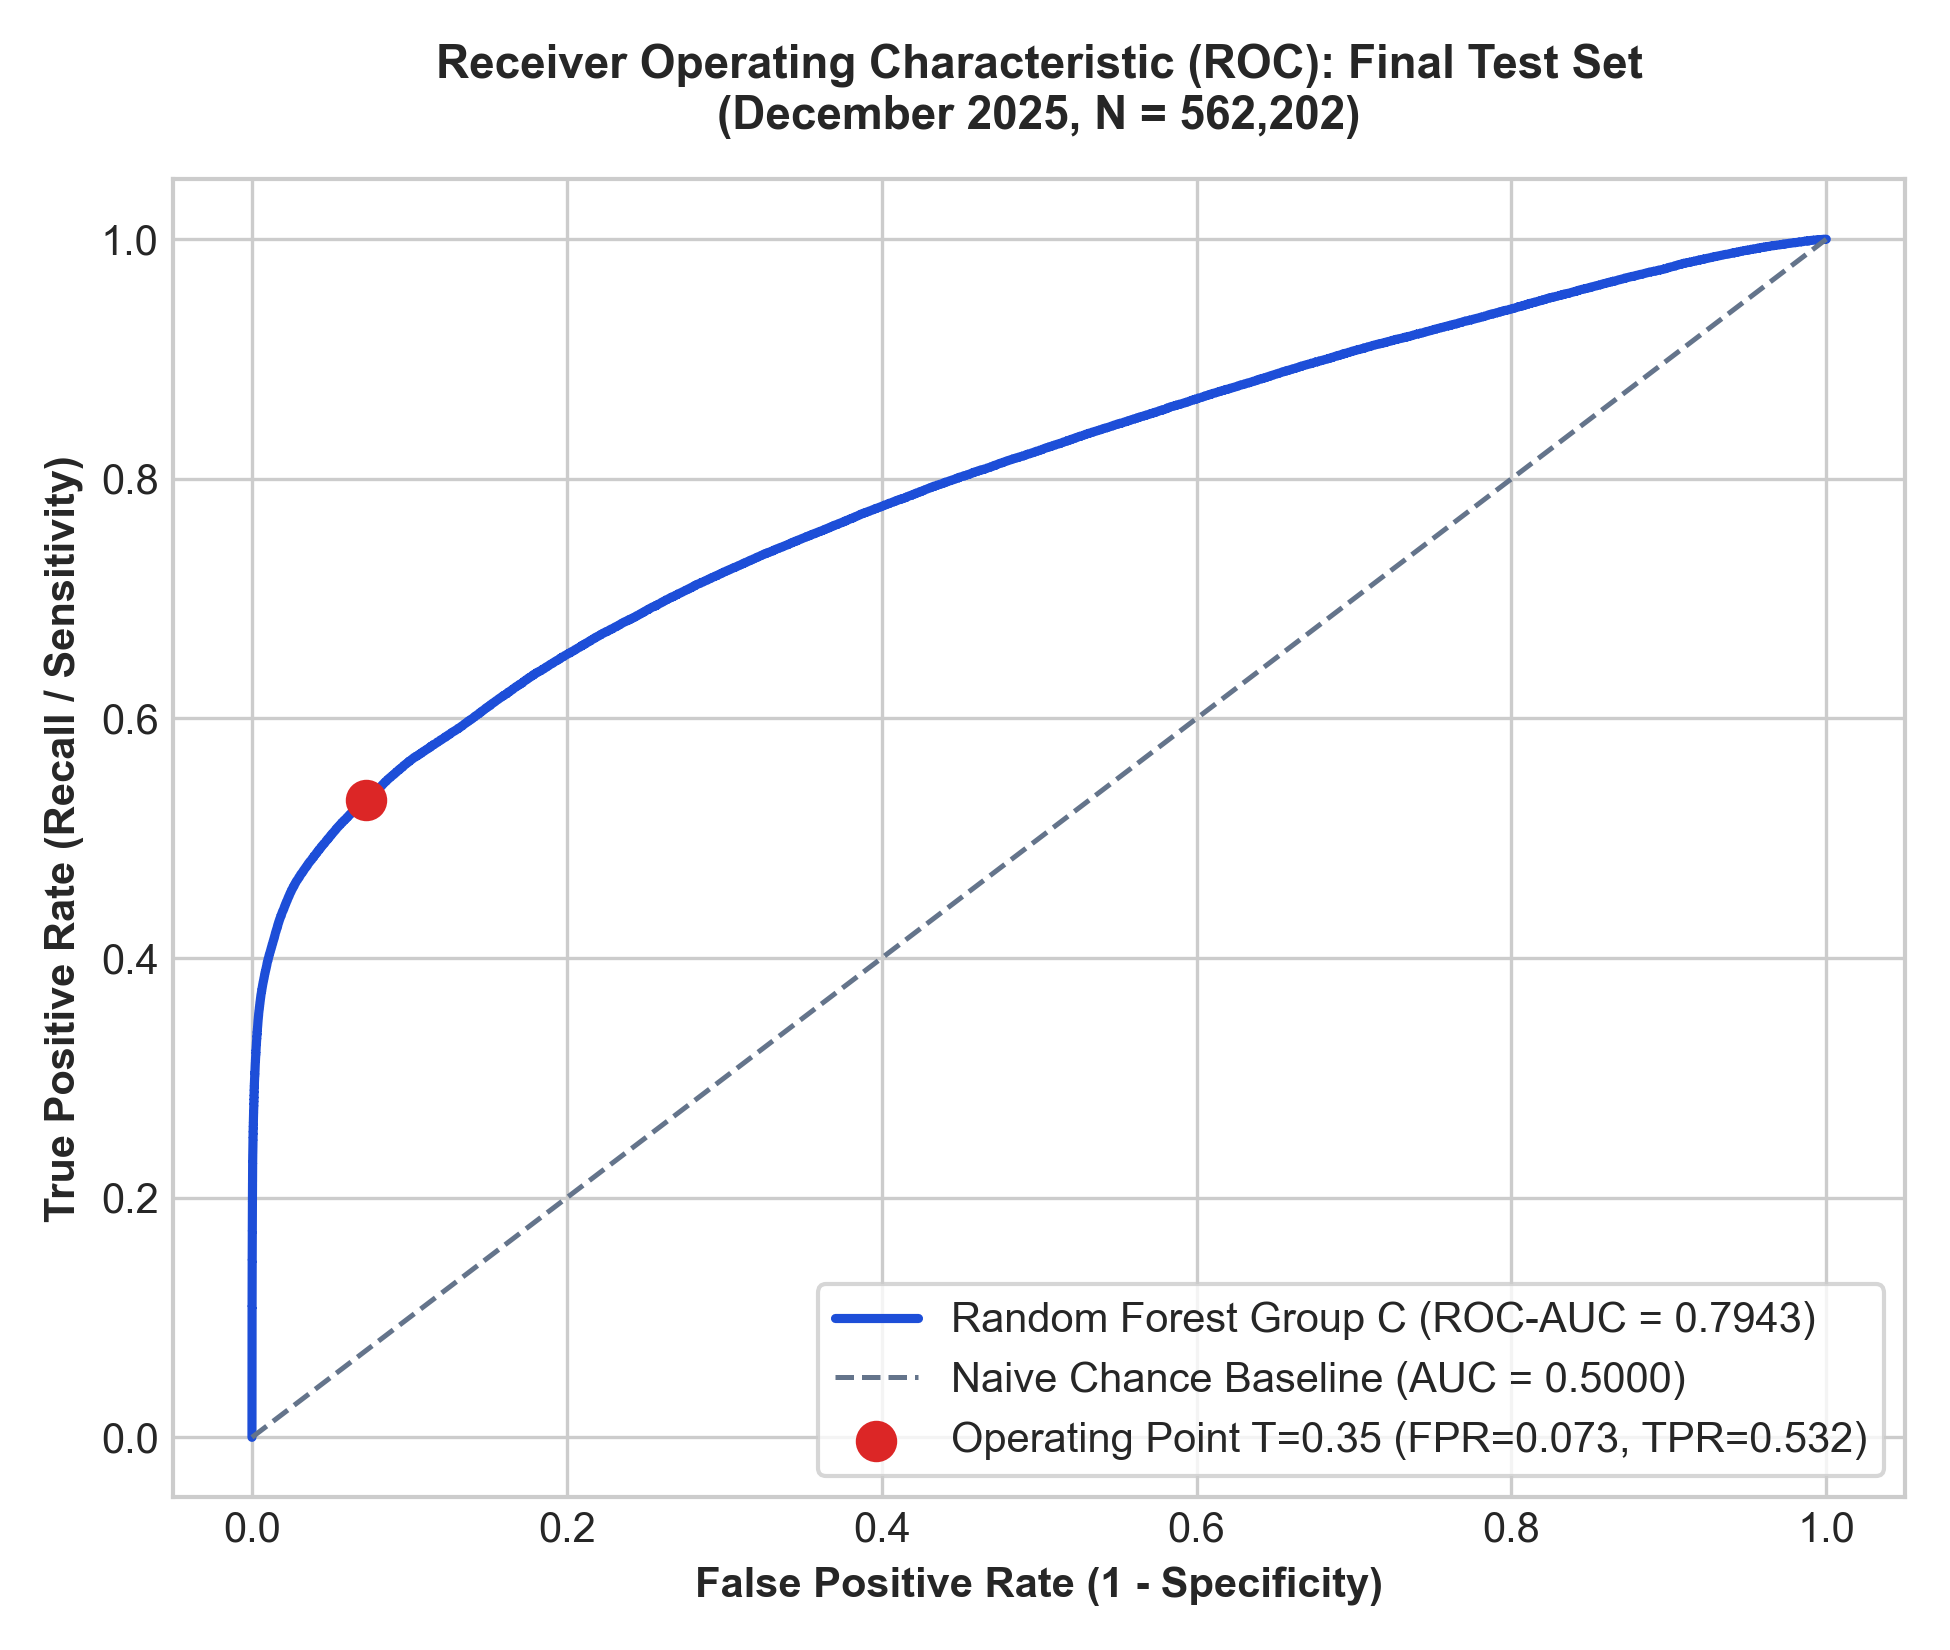
\includegraphics[width=0.46\columnwidth]{figures/fig_test_roc.png}\hfill
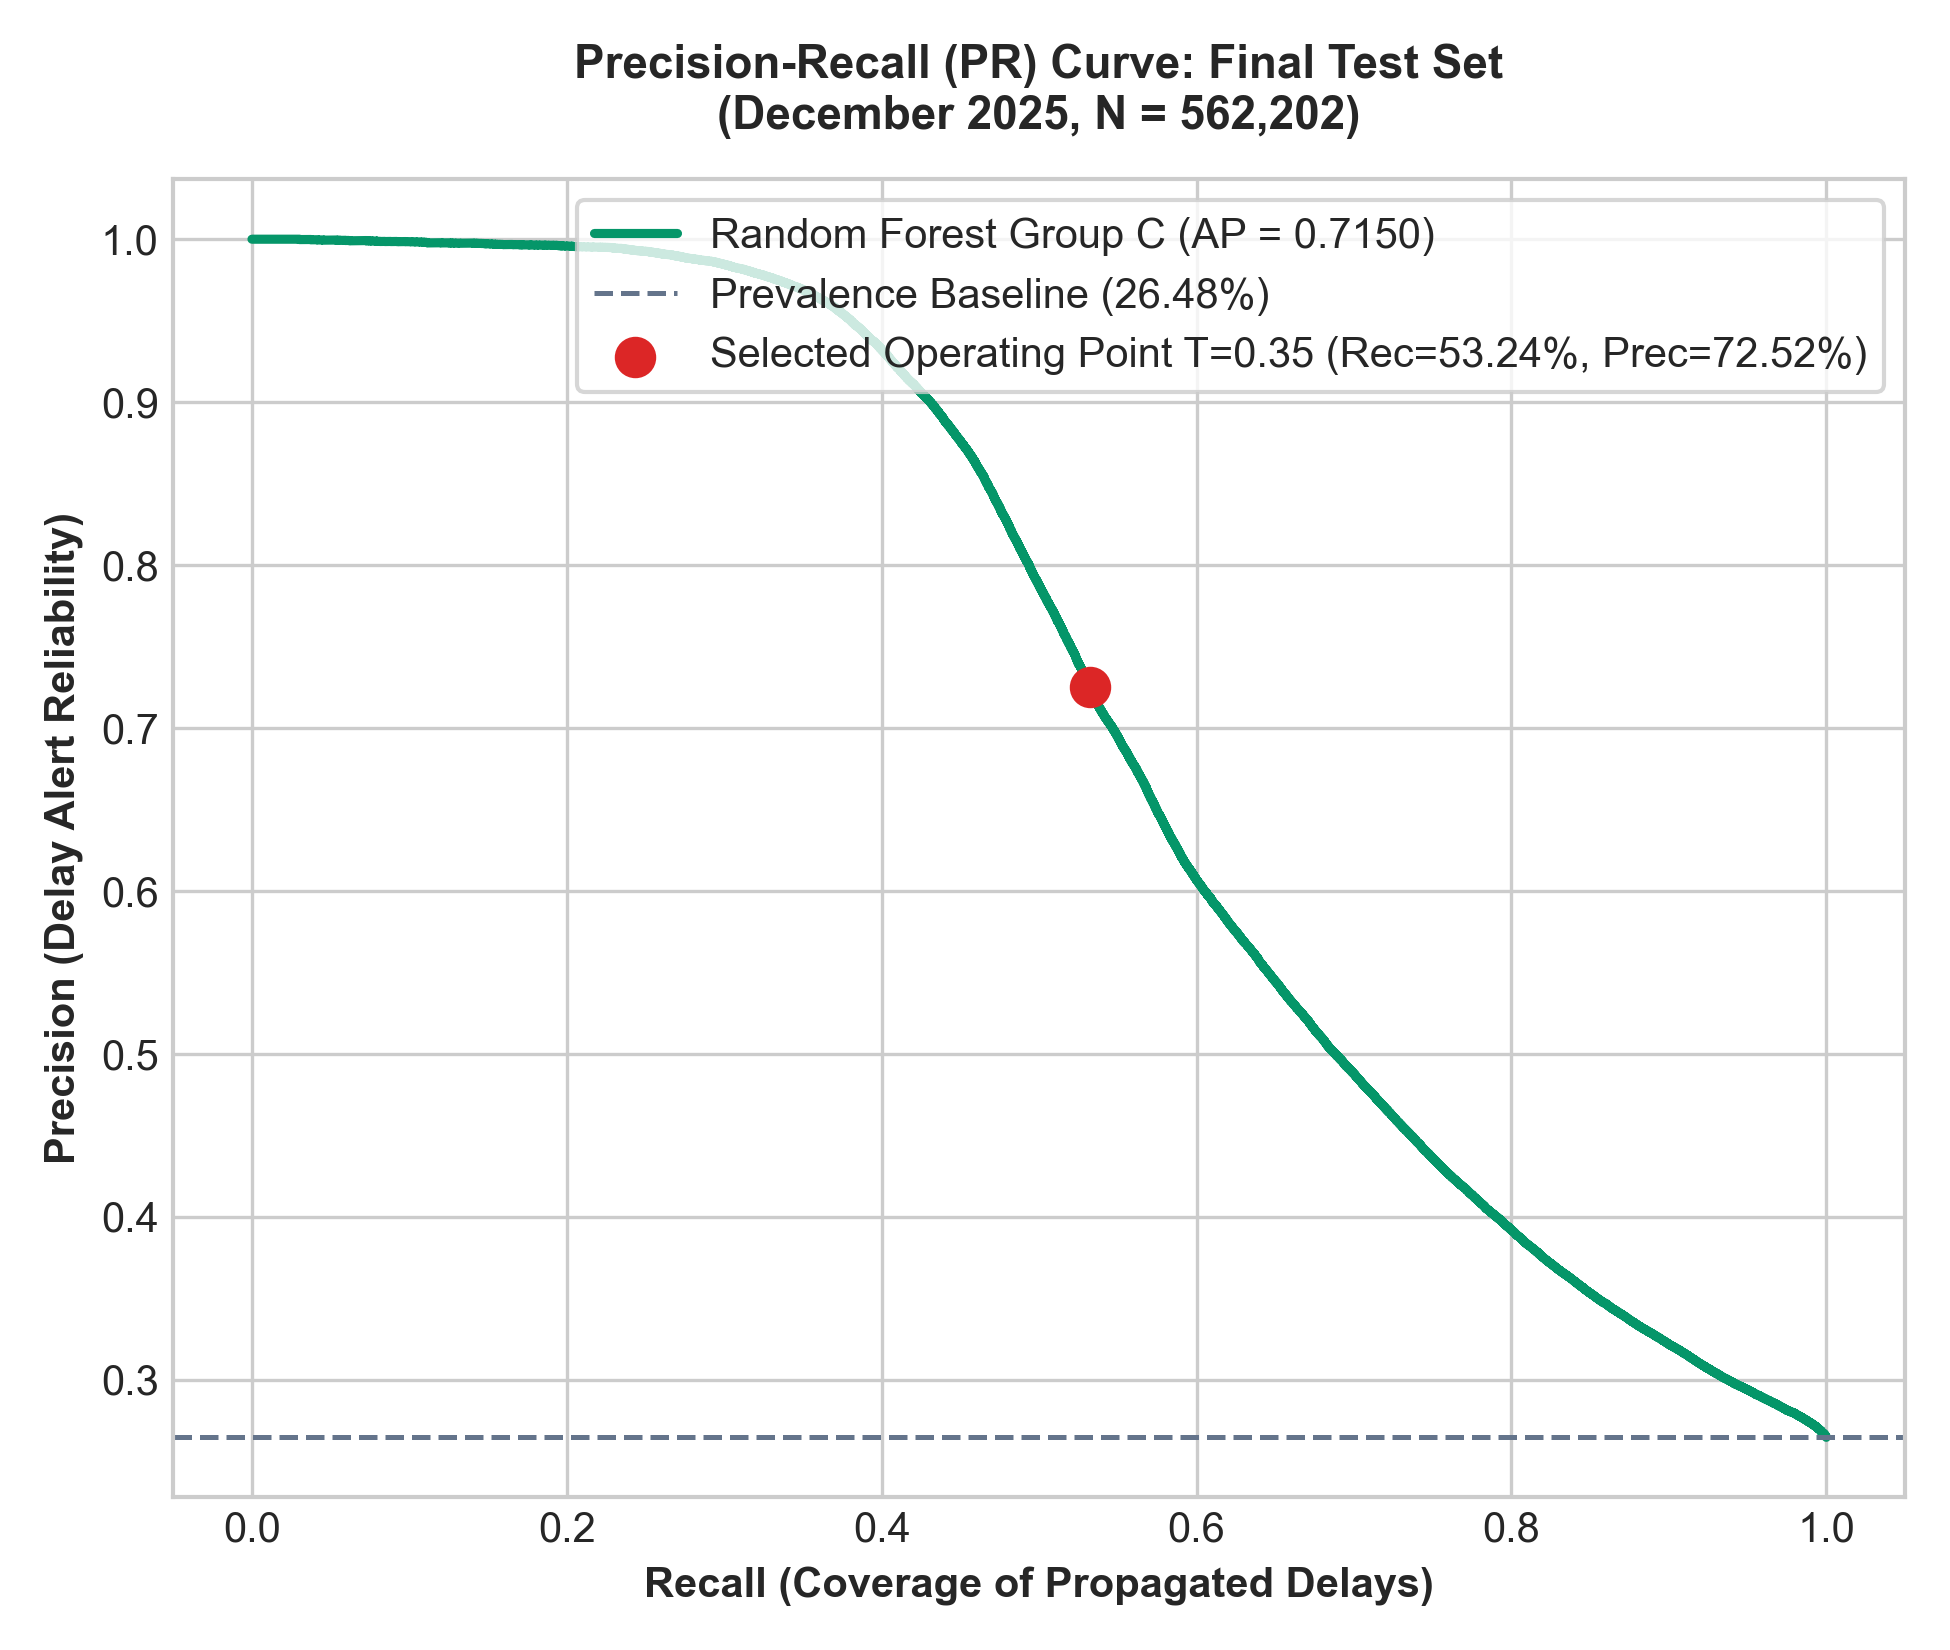
\includegraphics[width=0.46\columnwidth]{figures/fig_test_pr.png}
\caption{Classification performance on independent December test operations ($N = 562,202$). Left: ROC curve (AUC $= 0.7943$). Right: Precision-Recall curve (AP $= 0.7150$).}
\label{fig:test_discrimination}
\end{figure}

\begin{table}[t]
\caption{Out-of-Sample Generalization to December 2025 ($N = 562,202$)}
\label{tab:test_generalization}
\centering
\resizebox{\columnwidth}{!}{%
\begin{tabular}{lrrr}
\toprule
\textbf{Evaluation Metric}               & \textbf{Validation (Oct--Nov)} & \textbf{Test (Dec)} & \textbf{Change ($\Delta$)} \\
\midrule
\textit{Classification Discrimination}   &                                &                     &                            \\
ROC-AUC Score                            & 0.7932                         & \textbf{0.7943}     & +0.0011                    \\
Average Precision (AP)                   & 0.6600                         & \textbf{0.7150}     & +0.0550                    \\
Log Loss                                 & 0.3748                         & 0.4255              & +0.0507                    \\
\midrule
\textit{Operating Point ($T = 0.35$)}    &                                &                     &                            \\
Precision                                & 69.20\%                        & \textbf{72.52\%}    & +3.32\%                    \\
Recall                                   & 49.03\%                        & \textbf{53.24\%}    & +4.21\%                    \\
F1-Score                                 & 0.5740                         & \textbf{0.6140}     & +0.0400                    \\
Specificity                              & 94.47\%                        & 92.74\%             & -1.73\%                    \\
Overall Accuracy                         & 85.29\%                        & 82.28\%             & -3.01\%                    \\
\midrule
\textit{Continuous Regression}           &                                &                     &                            \\
Variance Explained ($R^2$)               & 0.4516                         & \textbf{0.4851}     & +0.0335                    \\
Mean Absolute Error (MAE)                & 17.40 min                      & 19.77 min           & +2.37 min                  \\
Root Mean Squared Error (RMSE)           & 38.62 min                      & 45.86 min           & +7.24 min                  \\
Unconditional Mean Bias ($y - \hat{y}$)  & +0.94 min                      & +1.21 min           & +0.27 min                  \\
\bottomrule
\end{tabular}%
}
\end{table}

\begin{table}[t]
\caption{Regression Residuals Across Delay Strata (Test Set)}
\label{tab:delay_bands}
\centering
\resizebox{\columnwidth}{!}{%
\begin{tabular}{lrrrrr}
\toprule
\textbf{Delay Stratum} & \textbf{Count} & \textbf{Share} & \textbf{MAE (m)} & \textbf{RMSE (m)} & \textbf{Bias (m)} \\
\midrule
Early / On-Time ($\le 0$m) & 322,255        & 57.32\%        & 13.01            & 16.69             & +12.27            \\
Minor Delay (1--14m)       & 91,082         & 16.20\%        & 10.58            & 12.64             & -3.46             \\
Moderate Delay (15--59m)   & 94,233         & 16.76\%        & 22.27            & 26.57             & -13.64            \\
Significant (60--119m)     & 31,939         & 5.68\%         & 42.70            & 54.03             & -30.78            \\
Severe Delay ($\ge 120$m)  & 22,693         & 4.04\%         & 109.98           & 201.18            & -90.38            \\
\midrule
\textbf{Aggregate Test Set}& \textbf{562,202}& \textbf{100\%}& \textbf{19.77}   & \textbf{45.86}    & \textbf{+1.21}    \\
\bottomrule
\end{tabular}%
}
\end{table}

\begin{figure}[t]
\centering
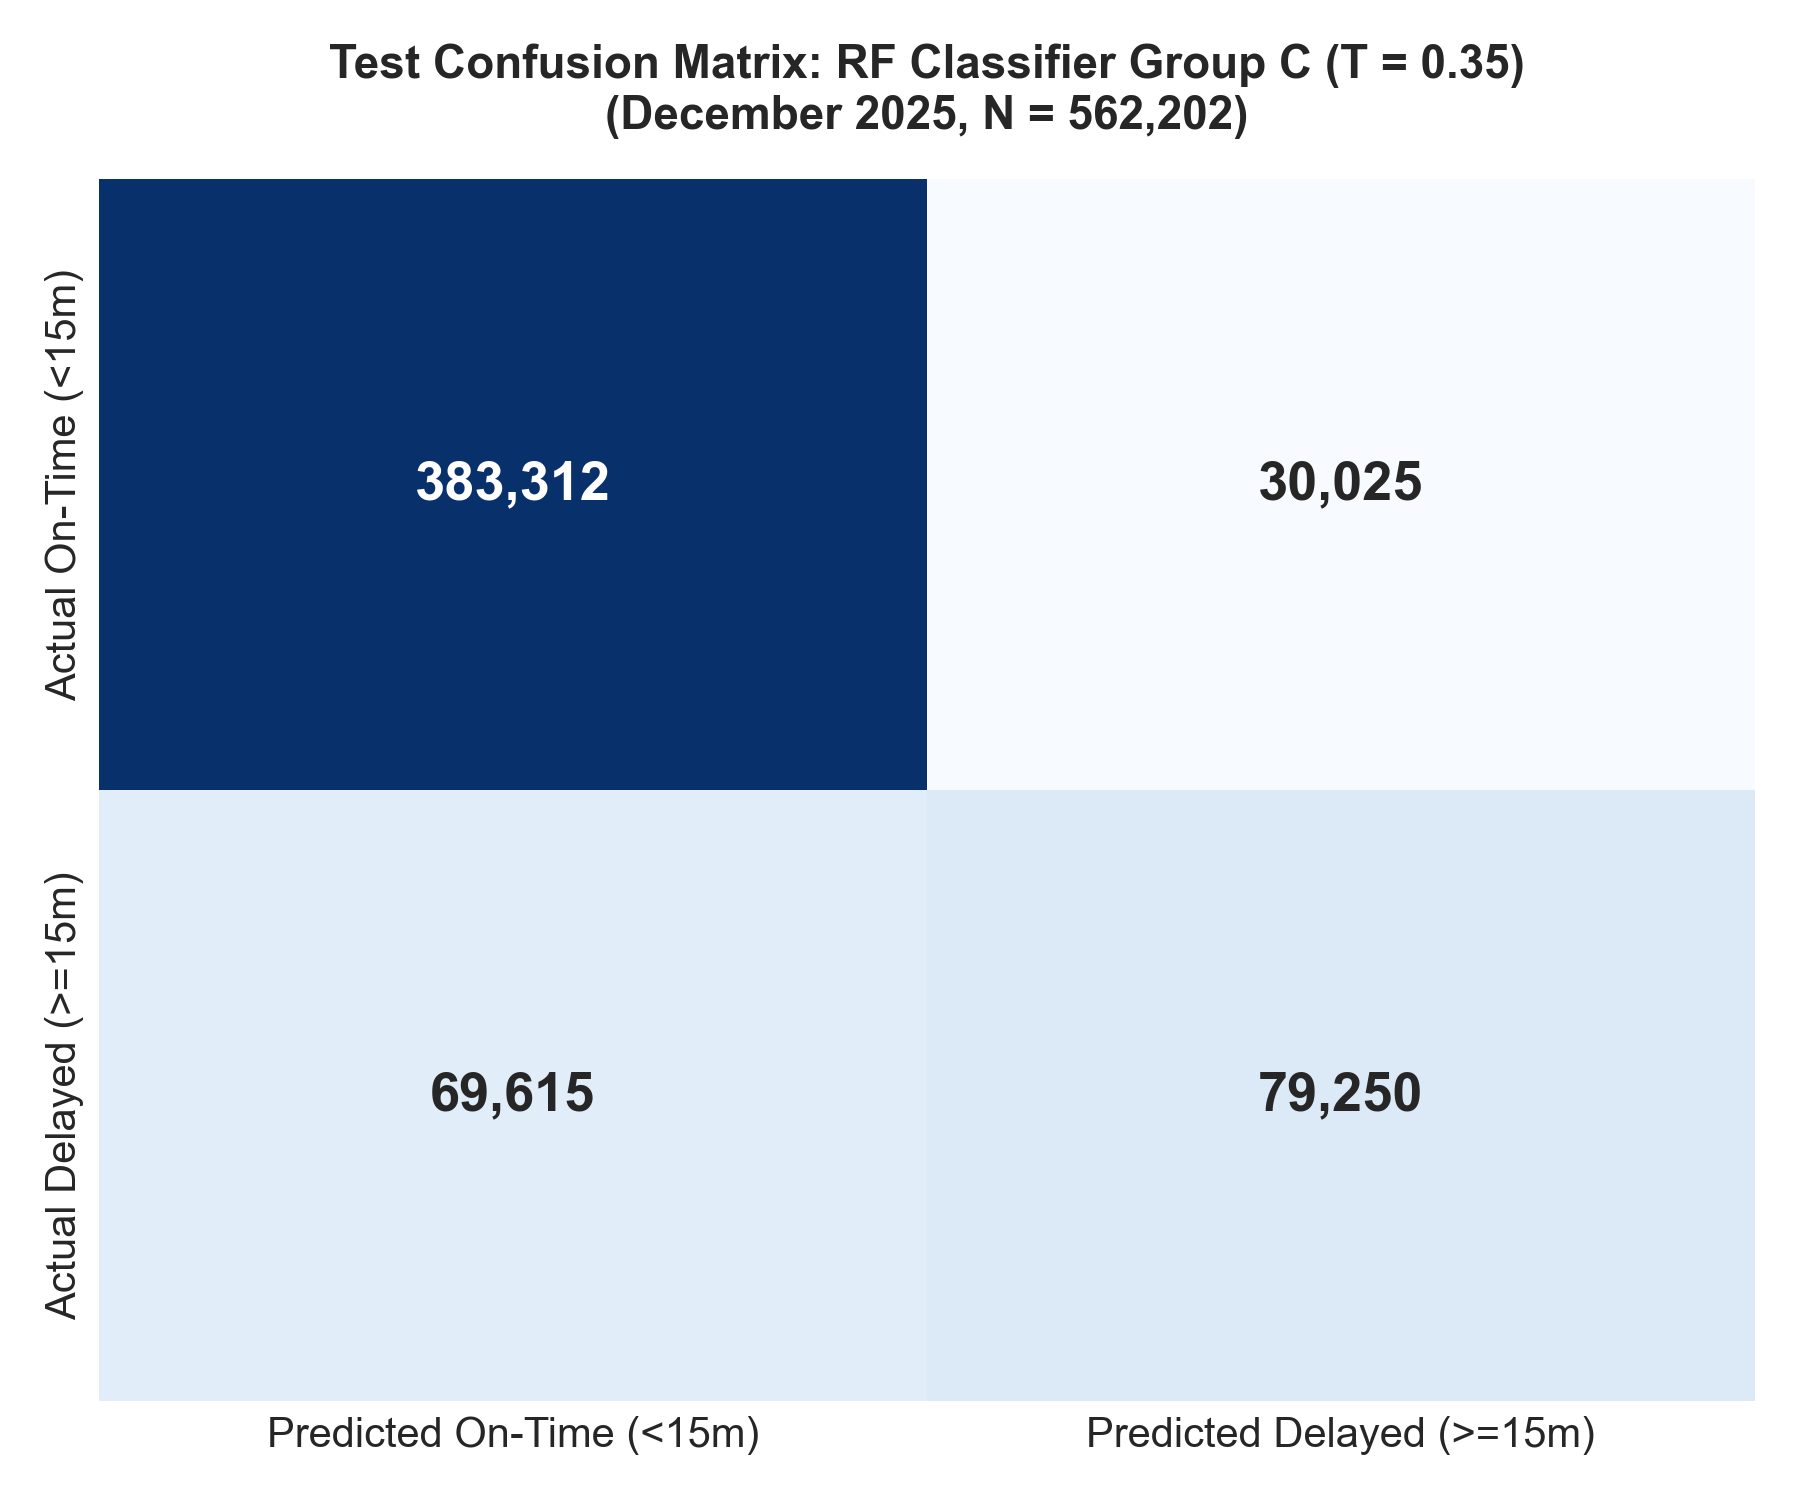
\includegraphics[width=0.46\columnwidth]{figures/fig_test_confusion_matrix.png}\hfill
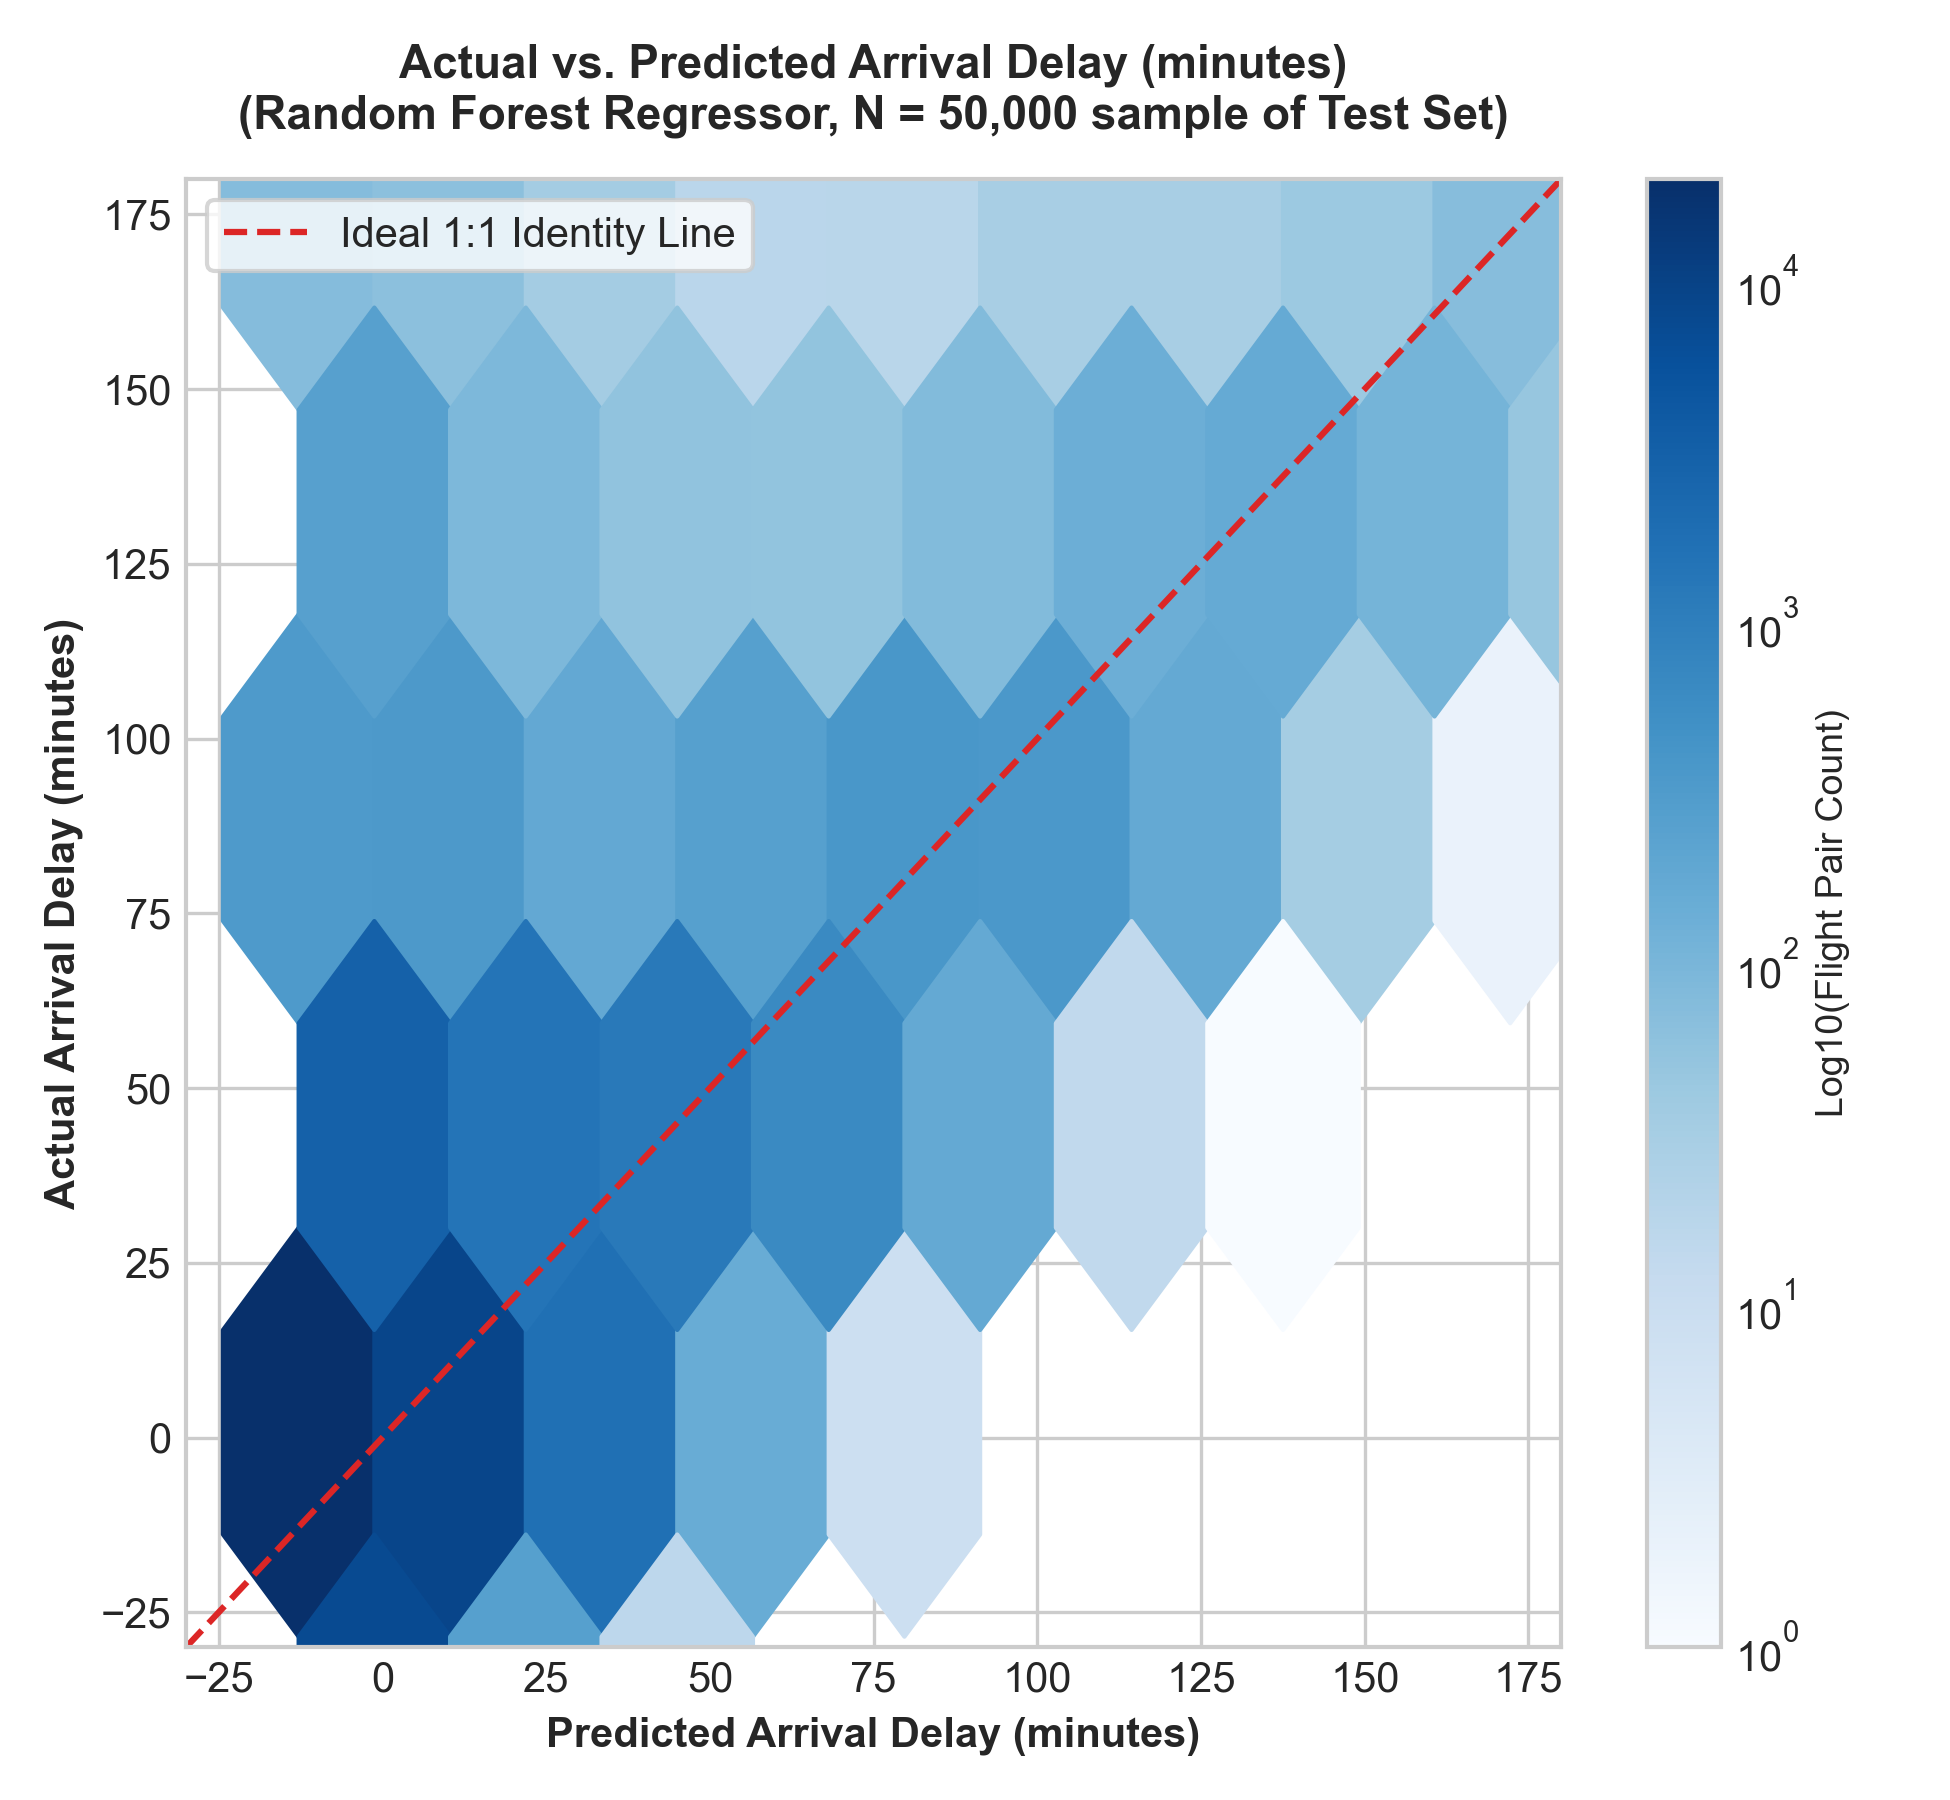
\includegraphics[width=0.46\columnwidth]{figures/fig_actual_vs_predicted.png}
\caption{Held-out December test evaluation ($N = 562,202$). (a) Confusion matrix for Random Forest Classifier at operational threshold $T = 0.35$. (b) Actual versus predicted arrival delay minutes for Random Forest Regressor ($R^2 = 0.4851$, $\text{MAE} = 19.77$m).}
\label{fig:test_dual_evaluation}
\end{figure}

\enlargethispage{3\baselineskip}
\subsection{Independent Test Generalization (December 2025)}
Evaluating frozen models on held-out December operations ($N = 562,202$) establishes robust out-of-sample temporal transfer (Table~\ref{tab:test_generalization}, Figs.~\ref{fig:test_discrimination} and~\ref{fig:test_dual_evaluation}):
\begin{itemize}
    \item \textbf{Classification Stability:} Discrimination transferred with zero decay: ROC-AUC was $0.7943$ (vs 0.7932 validation), and AP rose from $0.6600$ to $0.7150$ due to December's higher base delay prevalence (26.48\% vs 20.21\%).
    \item \textbf{Operational Dispatch at $T = 0.35$:} The model identified \textbf{53.24\% of all propagated delays} ($79,250$ true positives out of $148,865$ delayed flights) with \textbf{72.52\% precision}, while holding false alerts on on-time flights to \textbf{7.26\%} ($30,025$ false positives out of $413,337$ on-time flights; Fig.~\ref{fig:test_dual_evaluation}a).
    \item \textbf{Continuous Delay Explanation:} The regressor explained 48.51\% of total arrival delay variance ($R^2 = 0.4851$, $\text{MAE} = 19.77$ min), with an unconditional mean residual of $+1.21$ minutes.
\end{itemize}

\begin{figure}[t]
\centering
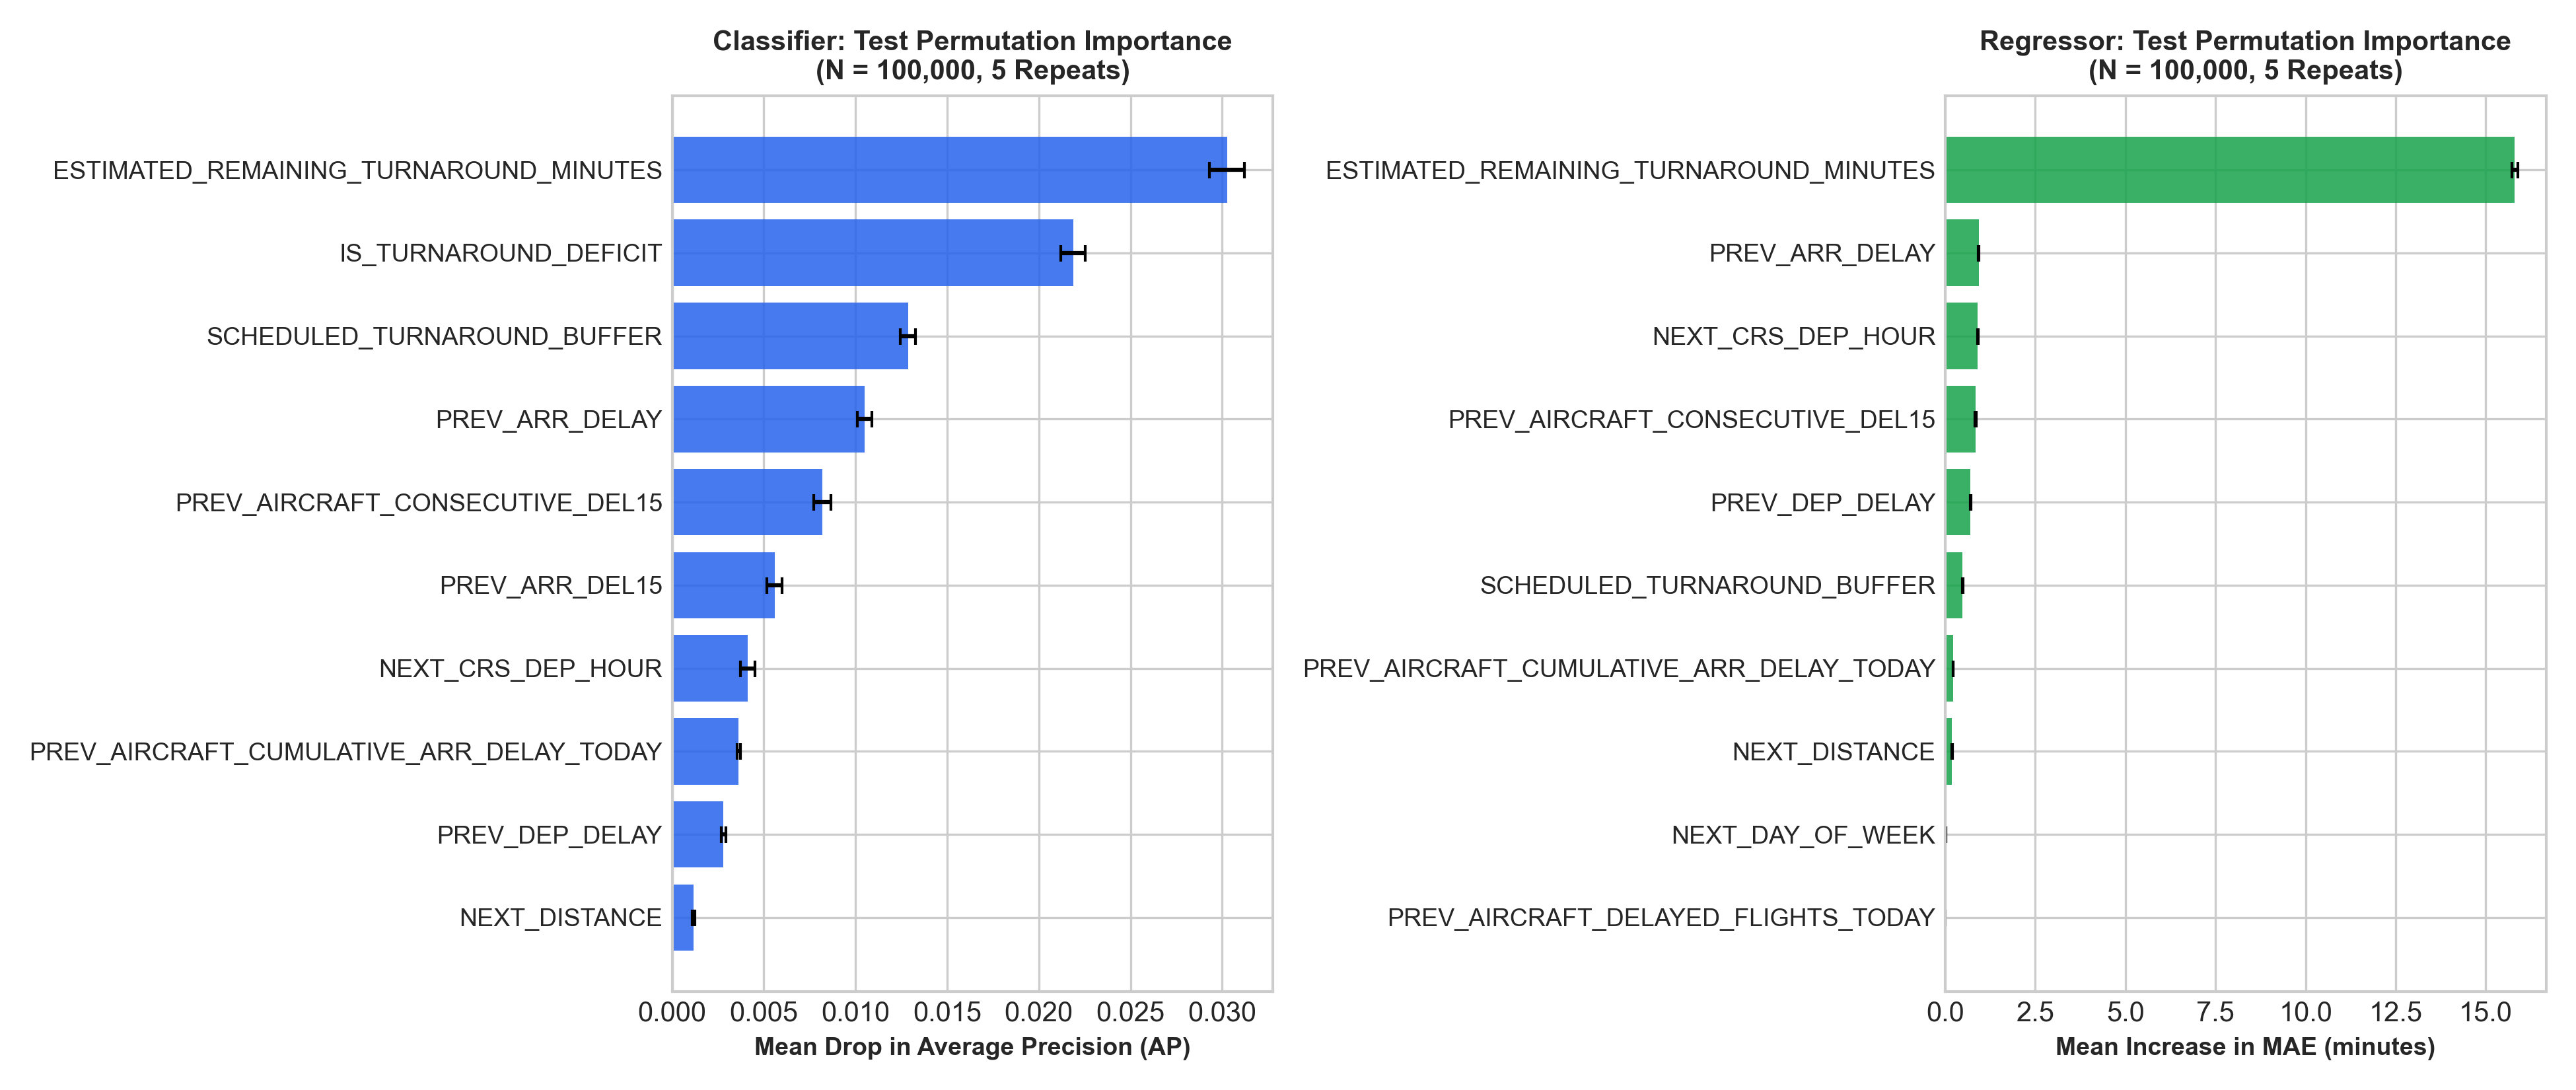
\includegraphics[width=0.78\columnwidth]{figures/fig_feature_importance.png}
\caption{Permutation feature importance on December test operations ($N = 100,000$, 5 repeats). Left: Drop in Average Precision. Right: Increase in MAE minutes.}
\label{fig:feature_importance}
\end{figure}

\subsection{Error Breakdown Across Operational Delay Regimes}
Stratifying test residuals across standardized operational bands reveals a clear operational dichotomy (Table~\ref{tab:delay_bands}):
\begin{itemize}
    \item \textbf{Ordinary Regimes ($\le 59$ min, 90.28\% of flights):} The model exhibits high predictive accuracy. For on-time flights ($\le 0$ min), MAE is 13.01 minutes; for minor delays ($1$--$14$ min), MAE is 10.58 minutes; for moderate delays ($15$--$59$ min), MAE is 22.27 minutes.
    \item \textbf{Severe Delays ($\ge 120$ min, 4.04\% of flights):} Errors rise sharply ($\text{MAE} = 109.98$ min, bias $= -90.38$ min). The actual mean delay in this cohort is $231.01$ minutes, whereas the model's conditional prediction averages $140.63$ minutes.
\end{itemize}

\subsection{Shift-Share Decomposition of Generalization Error}
Between validation and test, aggregate MAE increased from 17.40 to 19.77 minutes ($+2.37$ minutes). To investigate whether this reflects algorithmic degradation or seasonal population shift, we implemented the Oaxaca-Blinder / shift-share decomposition~\cite{oaxaca1973male,blinder1973wage}:
\begin{equation}
\Delta \text{MAE} = \sum_{i} w_{t, i} (e_{t, i} - e_{v, i}) + \sum_{i} (w_{t, i} - w_{v, i}) e_{v, i}
\end{equation}
where $w_i$ and $e_i$ denote stratum weights and MAEs. Under test weighting (Formulation A), the within-band error effect accounts for only \textbf{$+0.038$ minutes ($1.59\%$)}, while the composition shift effect accounts for \textbf{$+2.330$ minutes ($98.41\%$)}. Under symmetric Shapley weighting, composition accounts for \textbf{$93.99\%$ ($+2.225$ min)}. 

Crucially, in the moderate delay band ($15$--$59$ min), error actually declined by $-0.17$ minutes ($22.44 \rightarrow 22.27$ min). The macro-level error increase is mathematically attributable to the 55.4\% surge in severe disruptions ($\ge 120$ min) during winter travel, not model decay.

\subsection{Permutation Importance and Derived Identifiers}
Permutation importance on 100,000 test observations (5 repeats~\cite{fisher2019all}; Fig.~\ref{fig:feature_importance}) highlights the hierarchy of operational signals:
\begin{enumerate}
    \item \texttt{ESTIMATED\_}\allowbreak\texttt{REMAINING\_}\allowbreak\texttt{TURNAROUND\_}\allowbreak\texttt{MINUTES} ranked as the top predictor across both tasks (+0.0303 AP drop, +15.81 min MAE increase, $+0.9185$ $R^2$ drop).
    \item \texttt{IS\_TURNAROUND\_DEFICIT} was the second most critical classifier feature (+0.0219 AP drop).
    \item Airframe history features proved highly informative: \texttt{PREV\_}\allowbreak\texttt{AIRCRAFT\_}\allowbreak\texttt{CONSECUTIVE\_}\allowbreak\texttt{DEL15} ranked 5th overall (+0.0082 AP drop, +0.84 min MAE increase).
\end{enumerate}

\textit{Methodological Caveat on $R^2$ Drop:} For $\text{RemTurn}$, permuted model $R^2$ collapsed to $-0.4415$, producing an arithmetic drop of $0.4770 - (-0.4415) = +0.9185$. Because $\text{RemTurn}$ is an algebraic identity ($\text{Buffer} - \text{PrevDelay}$), univariate permutation creates impossible feature combinations that disrupt tree decision paths. This metric confirms the model's structural reliance on this derived representation, rather than an independent physical causal effect.

\section{Threats to Validity and Limitations}
Several scientific limitations qualify these findings:
\begin{enumerate}
    \item \textbf{Observational Association vs Causation:} Finding that buffer deficits predict delays does not prove that adding ground padding will causally eliminate downstream delays in a 1:1 ratio, as carriers adjust operational pacing in response to schedule buffers.
    \item \textbf{Unobserved Confounders:} BTS data omits real-time meteorological radar, de-icing queues, airport surface holds, and FAA Ground Delay Programs (GDPs)~\cite{faa2024atcscc}. These remain unobserved operational hypotheses.
    \item \textbf{Severe Tail Enclosure:} Random Forest regression predictions are bounded by conditional sample averages in terminal leaves (\texttt{min\_samples\_leaf=50}). While individual leaves output predictions up to $1,141.15$ minutes and test predictions reach $1,027.9$ minutes, the model cannot foresee extreme multi-hour compounding disruptions that occur post-departure.
\end{enumerate}

\enlargethispage{2\baselineskip}
\section{Conclusion and Future Work}
This research investigated the extent to which prior flight delays propagate across consecutive aircraft operations. Using 6.77 million commercial rotations reconstructed from BTS 2025 records, we demonstrated that incoming delays possess strong, statistically reliable predictive power for subsequent flights ($R^2 = 0.4851$, ROC-AUC $= 0.7943$). Turnaround buffer deficits represent the single most important operational bottleneck, while airframe rotational history provides non-redundant predictive signal.

An operational decision threshold of $T = 0.35$ provides airline operations control centers with an effective dispatch warning tool, capturing 53.24\% of propagated delays with 72.52\% precision. Future research will integrate real-time meteorological radar and crew schedule constraints to improve resolution in severe delay regimes.

\bibliographystyle{IEEEtran}
\bibliography{references}

\end{document}

